\documentclass[a4paper,oneside]{book}

% Use arial math font
\usepackage{arev}	
%\usepackage[mathcal]{euler}

%\usepackage[mathcal]{euler}
%\usepackage{mathpazo}
\usepackage[cm-default]{fontspec}
\usepackage{url}
\usepackage{hyperref}

\setmainfont[Mapping=tex-text]{Arial}
\setsansfont[Mapping=tex-text]{Arial Black}
\setmonofont[Mapping=tex-text]{Courier New}

%\setmainfont[Mapping=tex-text]{Hoefler Text}
%\setsansfont[Mapping=tex-text]{Optima}
%\setmonofont{Courier}

\usepackage{latexsym}
\usepackage{amsmath}
\usepackage{amssymb}

\usepackage{array}
\usepackage{longtable}

\usepackage{multirow}

\usepackage{graphics}

\usepackage{enumerate}

\DeclareMathOperator{\var}{Var}

% set page margins
\usepackage[margin=2cm]{geometry} 

\usepackage{color}

%\definecolor{mygray}{rgb}{0.5,0.5,0.5}
\definecolor{uwsblue}{cmyk}{0.96,0.41,0,0.43}

% set sans font to section headings
\usepackage{sectsty}
\allsectionsfont{\sffamily}
\sectionfont{\color{uwsblue}\sffamily}
\chapterfont{\raggedleft\color{uwsblue}\sffamily}

\renewcommand{\chaptername}{Section}

\setcounter{secnumdepth}{1}

%\newcommand{\vuws}{\textit{v}UWS}
\newcommand{\vuws}{vUWS}

\newcommand{\unitcode}{300958}
\newcommand{\unitname}{Social Web Analytics}

\newcommand{\teachingsession}{Spring}
\newcommand{\teachingsessiondate}{25th of February}
\newcommand{\teachingyear}{2013}
\newcommand{\intersessionbreak}{16th of April}

%\newcommand{\teachingsession}{Spring}
%\newcommand{\teachingsessiondate}{26th of July}
%\newcommand{\teachingyear}{2010}
%\newcommand{\intersessionbreak}{20th of September}

\newcommand{\goodfridaydate}{29th of March}
\newcommand{\goodfridayweek}{5}
\newcommand{\eastermondaydate}{1st of April}
\newcommand{\eastermondayweek}{6}
\newcommand{\anzacdaydate}{25th of April}
\newcommand{\anzacdayweek}{9}

\newcommand{\labourdaydate}{4th of October}
\newcommand{\labourdayweek}{11}
\newcommand{\publicholidays}{
There are three public holidays
this semester Good Friday (\goodfridaydate~\teachingyear, during week
\goodfridayweek), Easter Monday (\eastermondaydate~\teachingyear,
during week \eastermondayweek), and Anzac Day
(\anzacdaydate~\teachingyear, during week \anzacdayweek).}
%\newcommand{\publicholidays}{
%There is one public holiday
%this semester, Labour Day (\labourdaydate~\teachingyear, during week
%\labourdayweek).}


\newcommand{\timetablelink}{\url{http://platformweb.uws.edu.au/pweb_tt/start.asp}}


\newcommand{\HRule}{\rule{\linewidth}{0.2mm}}

\setlength{\parindent}{0in}
\setlength{\parskip}{0.7em plus 0.5em minus 0.2em}


\begin{document}



\begin{titlepage}
 
\begin{flushright}
\scalebox{0.2}{
\includegraphics{uws_cymk.pdf}}
\end{flushright}
\vspace{2em}
{\huge \unitcode~\unitname} \\
\HRule \\[1em]
{\Large School of Computing, Engineering and Mathematics}%\\[1em]
%\scalebox{0.57}{\includegraphics{cover-image}} \\[1em]
\begin{center}
%\scalebox{0.55}{\includegraphics{768px-Internet_map_1024}}
\scalebox{5}{
\includegraphics{Koala_Country_BBS_Login_Screen}} %\\[1em]
\end{center} %\\[1em]
\vspace{1em}
\begin{flushright}
%\fontsize{40}{40}
\fontspec[Scale=1.5]{Arial Black}
{\Huge  Learning Guide} \\[1em]
{\Huge \teachingsession~\teachingyear} \\[1em]
\end{flushright}
\vfill
\noindent
\HRule
 
\end{titlepage}

~
\vfill
\noindent
Cover image by Warrenlead taken from
\url{http://en.wikipedia.org/wiki/File:Koala_Country_BBS_Login_Screen.jpg}
is distributed under the Creative Commons Attribution-Share Alike 3.0 Unported 
license. Details of the licence can be found at
\url{http://creativecommons.org/licenses/by-sa/3.0/deed.en}

\newpage

\tableofcontents

\chapter{About \unitname}

\section{An introduction to this unit}

%<Insert information about the unit, for example the objectives of the unit>

The Social Web provides everyone with an elegant platform to voice
their opinion. The rapid take up of Web based social networking tools
by society has lead to an abundance of data containing the opinions of
millions of individuals.  Therefore, the analysis of information from
Facebook, Twitter and Google+ should allow us to identify trends and
relationships in society. Whilst this has interest on a personal
level, the killer­app will be in analysing such data for business;
tracking the buzz around a new product, understanding the links
between customers etc. This unit will introduce its students to the
Social Web data that is available, and blend computational,
mathematical and statistical concepts to allow extraction and analysis
of such data.

This Level 3 unit introduces students to various mathematical and
statistical techniques supporting the study of computing, engineering
and science. Presentation of the content will emphasise the correct
principles and procedures for accessing social Web data, performing
and understanding exposure analysis, analysing and visualising social
relationships using graphs, identifying important information using
text mining, and investigating the significance of trends. Topics
include graph analysis, text mining, temporal and spatial analysis,
and exposure analysis.


\unitname~is a core unit within the Bachelor of Information and
Communications Technology. 

Thus unit has the following prerequisites:
\begin{itemize}
\item 300700 Statistical Decision Making
\end{itemize}


% \section{Approach to teaching}
% This unit enhances learning through the following means:
% For example
% you  might like to state what the learning activities are, and how they contribute to student learning 
% how is feedback given
% etc


%This diagram can be deleted/modified to your requirements

\section{Staff details}
\begin{tabular}{ll}
  \textbf{Unit Coordinator:}  & Dr Laurence Park (first point of
  contact) \\
  & Building EN, Room 1.32, Campus: Parramatta \\
  & Phone: (02) 9685 9065 \quad
  Email: \texttt{l.park@uws.edu.au} \\[0.5em]

  \textbf{Teaching Staff:} & Assoc. Prof. Glenn Stone \\
  & Building EN, Room 1.31, Campus: Parramatta \\
  & Phone: (02) 9685 9253 \quad
  Email: \texttt{g.stone@uws.edu.au} \\[0.5em]

  \textbf{Tutors:} & Attila Egri-Nagy \\
  & Email: \texttt{a.egri-nagy@uws.edu.au} \\[0.5em]

  & Don Shearman \\
  & Email: \texttt{d.shearman@uws.edu.au} \\[0.5em] 
  
  & Kingsley Agho \\[0.5em] 

  & Nima Ramezani \\[0.5em] 

  & Shatha Aziz
\end{tabular}


\section{Student consultation arrangements}

Student consultation times will be arranged during the first week of
lectures and placed in the \unitcode~\unitname~section of \vuws.

\section{Essential Equipment}

\begin{itemize}
\item Calculator - A business or scientific calculator is essential
  for completing the exercises, test and exam.
\item Computer software - When carrying out the team project, you are
  required to use a computer using appropriate software, e.g. R, Excel to
  carry out all calculations and statistical analyses.
\end{itemize}
  
\section{Student feedback and improvements to the unit}

The University values student feedback in order to improve the quality
of its educational programs. If you wish to provide feedback, please
contact one of the staff listed above.


\chapter{You and this unit}

\section{What is expected of you}


\subsection*{Unit credit points and Workload}
This unit is a 10 credit point unit and will require your full and
continuous attention to maintain the highest possible grades.  It is
expected that you will spend at least 10 hours each week (on average)
which includes the four (4) contact hours per week.  Some weeks you
will spend more time on learning activities and assessments and in
other weeks the workload will be somewhat less.  It will be essential
for you to keep up with the assigned reading so that you are properly
prepared for each session.

\subsection*{Attendance}
Students are expected to attend the two hour lecture and a two
hour computer lab each week.

\subsection*{Online learning}
Students should access \vuws~to obtain lecture notes and information,
and check their student email account at least twice a week.

\subsection*{General conduct and behaviour}

According to the UWS Teaching and Learning code
(\url{http://policies.uws.edu.au/view.current.php?id=00139}) you are
required to:
\begin{itemize}
\item obtain the unit outline for this unit, by the end of the second
  teaching week;
\item regularly and actively participate in all scheduled educational
  activities, which includes lectures, tutorial, laboratory sessions,
  online activities etc;
\item give honest, helpful and courteous feedback to your lecturer(s);
\item make every effort to undertake the work required to successfully
  complete this unit;
\item submit work that is your own for any assessment task;
\item not indulge in any behaviour that disrupts the teaching and
  learning environment, or negatively affects fellow students and
  university staff, and understand that the University will take
  action against such behaviour as outlined in the Misconduct -
  Students Non-Academic Misconduct Policy;
\item treat university property with due care and report and damaged
  or broken equipment.
\end{itemize}
In addition, you should:
\begin{itemize}
\item be on time to lectures, tutorial and laboratory sessions.  If
  you are late, then please enter the lecture/tutorial room or lab
  with courtesy and consideration for others;
\item pay attention in lectures ,tutorials and laboratory sessions as
  this is where helpful information is given out of the assessment
  tasks;
\item switch off your mobile phone
\item ask questions about the content that you found difficult,
  immediately after the lecture, tutorial or lab session finishes.  If
  this cannot be accomplished, then make sure you see your lecturer or
  tutor as soon as possible to resolve any problems.
\end{itemize}


\section{What you can expect from the teaching team}

\subsection*{Feedback}

We will provide you with oral and written feedback on class test papers
immediately following the class in which they were presented.  You
will also receive feedback before you submit, and after handing in
your assignment questions.

\subsection*{Consultation}

There will be a weekly consultation time allocated in the first week
of the semester. Appointments can be made outside of the consultation
time via email.


\subsection*{General conduct and behaviour}

It is our aim to create a learning environment so that you may
reach your full potential in this unit.  Accordingly, you can expect
from the lecturing staff in this unit to:
\begin{itemize}
\item prepare thoroughly for each teaching session;
\item be on time for each lecture, tutorial and laboratory session;
\item ensure that you understand the unit requirements and material;
\item be available to assist students during the consultation times
  (as indicated above);
\item treat you equitably, and with courtesy and respect;
\item report immediately, any issues or concerns related to student
  academic and non-academic misconduct to the relevant authority,
  according to the UWS Misconduct Policy.
\end{itemize}
Sometimes the best laid plans do go astray!  In the unlikely
occurrence of this happening, you will be notified about any changes
to the scheduled activities, at least 24-hours in advance (if
possible), via an announcement on \vuws.

\section{How to use this learning guide}

This Learning Guide supplements the Unit Outline and is designed to
help you navigate through the unit.  It will help you focus on what
you need to do to prepare for the various assessment tasks throughout
the unit.  You should consult the Learning Guide on a regular basis,
as you plan your study, as this guide contains information on how best
to prepare for each assessment task.

The Learning Guide also offers tips to assist you in developing the
skills and techniques of an effective, independent learner.  However,
if you have any particular problems or issues regarding this Unit,
please take these up with the Unit Coordinator so that they may be
resolved as soon as possible.  As an adult learner, it is expected
that you will be responsible for your own learning and take the
necessary and appropriate steps to ensure your success.

\section{Policy and how it affects you}

The University has a number of policies that relate to teaching and
learning.  Important policies affecting students include:
\begin{itemize}
\item Assessment Policy
\item Examinations Policy
\item Special Consideration Policy
\item Review of Grade Policy
\item Assessment Practice - Fundamental Code
\item Misconduct - Student Academic Misconduct Policy (see extract of
  the policy below under the heading "What is Academic Misconduct?")
\item Misconduct - Student Non-academic Misconduct Policy
\item Enrolment Policy (includes a section on the UWS Student Email Account)
\item Bullying Prevention Policy and Guidelines
\item Sexual Harassment Prevention Policy
\end{itemize}
There are two policies that relate to misconduct - academic and
non-academic misconduct.  Breaches of these policies can have very
serious consequences.  It is essential that you are familiar with
these policies and how to ovoid misconduct of any type.


\subsection*{What is Academic Misconduct?}

Academic Misconduct may involve plagiarism, collusion or cheating.
Plagiarism involves submitting or presenting work in a unit as if it
were the student's own work when, in fact, it was not. Collusion
includes inciting, assisting, facilitating, concealing or being
involved in plagiarism, cheating or other academic misconduct with
others.  Cheating includes dishonest conduct (or attempted dishonest
conduct) in exams.

For the full definition of academic misconduct and the consequences of
such behaviour, you are advised to read the Misconduct - Student
Academic Misconduct Policy in its entirety, refer to:
\url{http://policies.uws.edu.au/view.current.php?id=00051} 

The School of Computing, Engineering and Mathematics definitions of Minor and
Substantial Breaches of the UWS Academic Misconduct policy are below:

\subsection*{Plagiarism}

Minor breach: A minor breach occurs when the weighting of the
assessment task is 10\% or less, and 20\% or less of the work
submitted is taken from another source without reference to the
original source or author.

Substantial breach definition:  A substantial breach occurs when:
\begin{enumerate}
\item Either the weighting of the assessment task is more than 10\%,
  or 20\% or more of the work submitted is taken from another source,
  without reference to the original source.
\item If a student has been found to have already committed an act of
  plagiarism and warned about it, whether it be a minor or substantial
  breach, then the next allegation will be treated as a substantial
  breach.
\end{enumerate}

\subsection*{Cheating}

\begin{enumerate}
\item  Dishonest or attempted dishonest conduct during an examination,
for example speaking to other candidates or otherwise communicating
with them, leaving answer papers exposed for other students to view
and/or copy or attempting to view another student's solutions, would
be deemed as minor.  However, if this behaviour continued after the
student had been asked to desist, then the breach would be treated as
substantial.

\item  Bringing into the examination room any textbook, notebook,
memorandum, other written material or mechanical or electronic device
(including mobile phones), or any item not authorised by the examiner
would be treated as minor.  However, if the student does not surrender
the unauthorised item, then a substantial breach would have occurred.

\item  Writing an examination or part of it, or consulting any person or
materials outside the confines of the examination room without
permission to do so, would constitute a substantial breach.

\item  Cheating in take-home examinations, which includes, but it not
limited to: making notes, papers or answers in connection with the
examination (in whatever form) to others without the permission of the
relevant lecturer; receiving answers, notes or papers in connection
with the examination (in whatever form) from another student, or
another source without the permission of the relevant lecturer; and
the unauthorised collaboration with another person or student in the
formulation of an assessable component of work constitutes a
substantial breach.
\end{enumerate}

\subsection*{Other Academic Misconduct}

\begin{enumerate}
\item Tampering or attempts to tamper with examination scripts, class
  work, grades or class records, will be regraded as substantial.

\item Failure to abide by the directions of an academic member of
  staff regarding the individuality of work to be handed in, will, in
  the first instance be treated as minor.  However, any recurrence
  of such behaviour will be regarded as substantial.

\item Acquisition, attempted acquisition, possession or distribution
  of examination materials or information without the authorisation of
  the academic member of staff will be regarded as substantial.

\item Impersonation of another student in an examination or other class
assignment will be regarded as substantial.

\item Falsification or fabrication of practical or laboratory reports
will be regarded as substantial.

\item Non-authorised use of tape recording of lectures will be regarded
as minor, except where the student/s has been asked to desist and
refuses to comply.  This continued abuse will be regarded as
substantial.
\end{enumerate}


There are many resources to help you ovoid academic misconduct.  The
library staff (see section \ref{sec:library}) can help you with referencing and the
Student Learning Unit can assist with academic writing and plagiarism.
If you are unsure about any of your work you should also ask your
tutor or lecturer for advice and feedback.

\subsection*{What is Non-academic Misconduct?}

Non-academic misconduct includes unlawful activities and crimes,
falsifying documents (like a medical certificate or academic records),
harassing other students (or staff), stealing or damaging university
property (like library books or computers) and disrupting other
students or staff.  These are just some of the types of non-academic
misconduct and while these things are rare they do happen.  If you
believe you have been the victim of non-academic misconduct or you are
aware of any academic misconduct it is very important that you report
it.


You should report all matters of academic misconduct directly to your
Head of Program.

\section{What to do if you have a problem/concern}

If you have a concern about this unit please contact the unit
coordinator in the first instance.  If you would prefer to speak to
someone else you are advised to contact your Head of Program (see the
online handbook to identify your Head of Program and their contact
details \url{http://handbook.uws.edu.au/hbook/}).

More information about resolving complaints is available on the UWS
website. \url{http://uws.clients.squiz.net/opq/planning_and_quality/complaints_management_and_resolution}.

The University also has a confidential Complaints Handling department
(see link above for contact details).  You may contact this department
of the University at any time however we would appreciate the
opportunity to resolve this directly first.




\chapter{Teaching and Learning Activities}

Details of the teaching resources and learning activities are provided
in this section of the learning guide.


\section{Schedule of Learning and Teaching Activities}
The \teachingsession~teaching session begins on \teachingsessiondate
\teachingyear.  The inter-session break begins on
\intersessionbreak~\teachingyear.  \publicholidays~
%  (for Autumn
% session.  Please put in the date for the October long weekend for the
% Spring session).  
%These public holidays will affect classes at Penrith. 
When classes
fall on public holidays, students are expected to revise the missed
material in their own time. In the case of a missed lecture, lectures
online will be available within \vuws.


\noindent
\renewcommand{\arraystretch}{1.3}
\begin{longtable}{|c|>{\raggedright}p{0.5\textwidth}|>{\raggedright}p{0.2\textwidth}|>{\raggedright\arraybackslash}p{0.15\textwidth}|}
\hline
Week & Topic & Text readings & Assessment \\
\hline
1 & Introduction to the Social Web  & & \\
\hline
2 & Introductory R programming and data structures &  & \\
\hline
3 & Simple Exposure Analysis &  & Online Test 1 \\
\hline
4 & Text Mining 1 (indexing, weighting, querying, metrics) &  &  \\
\hline
5 & Graphs 1 (Definition, Graph statistics, Storage) & &  Online Test 2 \\
\hline
6 & Visualisation &  &  \\
\hline                                            
7 & Text Mining 2 (Clustering) &  &  Online Test 3 \\
\hline                                            
8 & Graphs 2 (PageRank, HITS, Shortest Path) &  & \\
\hline
9 & Semester Break & &  \\
\hline                                             
10 & Time 1 (trends, trend periodicity)  & & Online Test 4 \\
\hline                                            
11 & Time 2 (BACI designs) &  & \\
\hline
12 & Text Mining 3 (Sentiment Analysis) &  & Online Test 5  \\
\hline
13 & Spatial Analysis &  & Group Project Due \\
\hline                                            
14 & Revision &  & \\                
\hline
\end{longtable}


Each week, students are expected to attend lectures and
computer labs. For full details about the timetable for this unit, go to
\timetablelink~and search for \unitcode.



\subsection*{Lectures}

Lectures are large classes where students are introduced to new ideas
and concepts. The notes presented in the lectures will be available in
the \unitcode~\unitname~section of \vuws.

%\subsection*{Tutorials}
%
%Tutorials are small classes where students work through questions and
%problems related to the lecture content. It is expected that students
%attempt the tutorial questions before coming to the tutorials.

\subsection*{Computer Labs}

Computer Labs are small interactive classes based in a computer lab where
the tutor will discuss how to use computers to assist us in
solving statistical problems. Time will be given in the labs for
students to work on problems with the assistance of the tutor.


\chapter{Assessment Details}

This section provides detailed information about the assessment
activities in this unit. You are encouraged to use this as a guide
when you are working on each assessment task.

\section{Assessment summary}

There are seven main assessment activities in this unit:
\begin{center}
\begin{tabular}{|l|>{\raggedright}l|>{\raggedright}l|>{\raggedright\arraybackslash}l|}
  \hline
  Component & Weighting & Date of Assessment & Content covered in
  week/s \\
  \hline
  Online Test 1 & 5\% & Week 4 & 1 and 2 \\
  Online Test 2 & 5\% & Week 5 & 3 and 4 \\
  Online Test 3 & 5\% & Week 6 & 4 and 5 \\
  Online Test 4 & 5\% & Week 7 & 5 and 6 \\
  Online Test 5 & 5\% & Week 8 & 6 and 7 \\
  Online Test 6 & 5\% & Week 10 & 7 and 8 \\
  Online Test 7 & 5\% & Week 11 & 8 and 10 \\
  Online Test 8 & 5\% & Week 12 & 10 and 11 \\
  Project           & 25\% & Week 13         & Various \\
  Final Examination & 50\% & During the exam period & 1 to 13 \\
  \hline
\end{tabular}
\end{center}
%\textbf{* The highest 3 marks from the 4 tutorial exercise sets will be taken.}

The compulsory assessment tasks are: participation in the final
examination. See below for further details. Students who do not
participate in this task will receive an automatic failing grade
(AF).
\begin{itemize}

\item An \textbf{absent fail}, AF grade is defined as: Student has not
officially withdrawn from the unit and has failed to complete one or
more of the compulsory assessment requirements for the unit.

\item A \textbf{compulsory fail}, CF grade is defined as: A student has
failed a compulsory component of a unit. If a student receives a CF
grade, they have failed the unit irrespective of the percentage mark
achieved.
\end{itemize}
In order to pass this unit you must obtain a minimum combined overall
mark of 50/100. No student, regardless of performance throughout the
session, should expect to attain a passing grade in this unit without
attaining;
\begin{itemize}
\item at least 40\% in the final examination.
%\item at least 40\% for the continuous assessment (tests and
%  assignment).
\end{itemize}
The following cut-off marks may act as a guide:
\begin{itemize}
\item High Distinction (H):            85/100 or higher
\item Distinction (D):                 75/100 - 84/100
\item Credit (C):                      65/100 - 74/100
\item Pass (P):                        50/100 - 64/100
\end{itemize}
In this unit learning and teaching activities consist of a weekly
two-hour lecture and a weekly two-hour computer lab. The computer lab
is designed to allow student to implement the ideas presented in the
lectures.



Students are expected to work individually through the set topics,
receiving assistance as required and attempting specific lab
tasks for each topic. Students should be aware that in this unit,
later topics build on the material covered earlier.


\section{Learning outcomes and assessment}


Students are expected to gain an understanding of the fundamental
concepts of Web social networks as well as the ability to apply modern
mathematical and statistical techniques to analyse the social network
properties.  On successful completion of this unit, students should be
able to:

\begin{center}
%\begin{tabular}{|>{\raggedright}p{0.4\textwidth}|>{\raggedright\arraybackslash}p{0.5\textwidth}|}
 \begin{tabular}{|>{\raggedright\arraybackslash}p{0.4\textwidth}|>{\raggedright\arraybackslash}p{0.5\textwidth}|}
%\begin{tabular}{ll}
\hline
\textbf{Learning Outcomes} & \textbf{Assessment Tasks} \\
\hline
Extract and process formatted data from social Web sources. &  \multirow{3}{0.4\textwidth}{Online Quizzes, Group Project} \\
\cline{1-1}
Use computer algorithms to visualise complex social Web interactions. & \\
\cline{1-1}
Partition a social network into clusters. & \\
\hline
Use mathematical and statistical methods to identify significant trends in the social Web. &  \multirow{3}{0.5\textwidth}{Online Quizzes} \\
\hline
Use mathematical and statistical techniques to identify critical regions of a social network. &  \multirow{3}{0.5\textwidth}{Online Quizzes, Exam, Group Project} \\
Choose an appropriate metric to measure the interaction between social network nodes. & \\
\cline{1-1}
Compute the popularity, authority and hub scores for network nodes. & \\
\hline
\end{tabular}
\end{center}

Each of the assessment tasks has been designed to evaluate the extent
to which you have achieved these learning outcomes.

\section{Assessment details}

The components of the assessment for this unit are as follows.
%\renewcommand{\arraystretch}{1.3}

\subsection*{Online Quizzes, best 5 of 8 @ 4\%, weighting 20\%}

The online quizzes will be short tests, expected to take 15 minutes
each, that will provide students a chance to assess their knowledge
throughout the unit.  There will be eight quizzes, but only the best
five of the eight will contribute towards the students final grade.

\subsection*{Group Project, weighting 30\%}

The group project is designed to examine if each student can apply the
knowledge from the unit to analyse a social network.  The project
will be completed with a group of students, therefore it is crucial
that all students in the team work together and delegate the tasks
effectively.

More information on this may be found on the \vuws~site.


\subsection*{Final Examination, weighting 50\%}

This is a compulsory assessment item. Students who do not attempt the
final (or deferred exam, if eligible) will be given an automatic
failing grade.

This assessment item has a 40\% hurdle, meaning that any student
obtaining fewer than 20 of the 50 exam marks will receive a compulsory
fail grade (CF) for their final mark.

This is an open book examination to determine whether you are able to
employ the appropriate mathematical and statistical methods and
techniques in given situations. It will be 2 hours in duration.



% The examination consists of three sections, A, B and C. Each section will consist of three
% questions. You should answer two questions in each section. If you answer three questions in a
% section only the first two questions will be marked. You must write down your working and
% answers in the answer books provided.

\subsection*{Calculation of Final Mark and Grade}




Marks and subsequent grades for \unitcode~\unitname~will be
calculated in one of the following way:
\begin{itemize}
\item
  Quizzes (20\%) + Group project (30\%) + Final Examination (50\%)
\end{itemize}



\subsection*{Examples of typical questions and typical answers that
  would achieve high, or perfect, scores.}






\subsubsection*{Question (4 marks)}

Plot the degree distribution of the following graph and identify if it
is a small world graph or not.
% g = barabasi.game(10, directed=FALSE)
% plot(g)
% table(degree(g))

\vspace{-6em}
\begin{center}
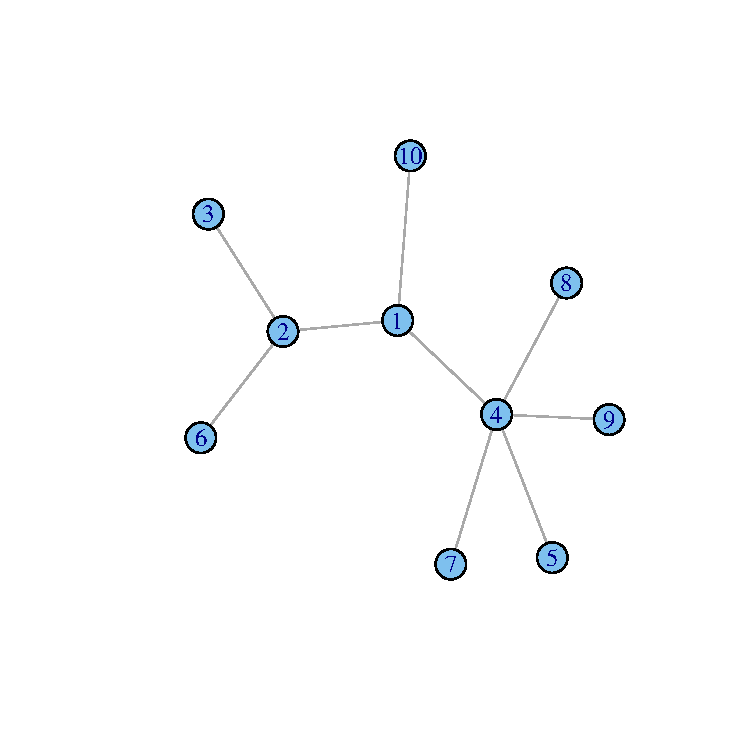
\includegraphics{bnetwork}
\end{center}

\subsubsection*{Solution}

The degree distribution is:
\begin{center}
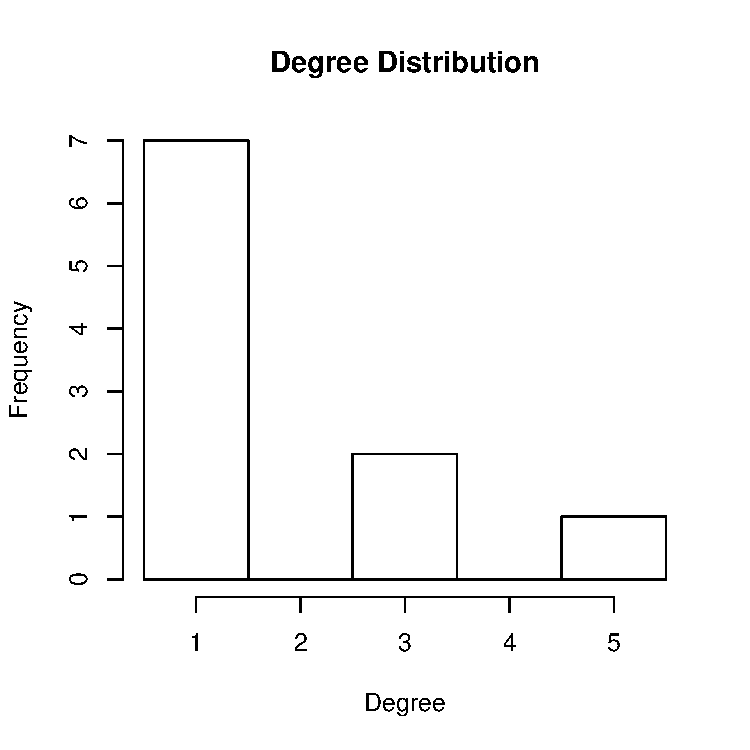
\includegraphics{bnetwork-dist}
\end{center}

The distribution shows that the frequency is exponentially decreasing
as the degree increases and so this graph resembles a small world
graph.


\subsubsection*{Question (4 marks)}

Using the following document set:
\begin{enumerate}
\item One one was a race horse.
\item Two two was one too.
\item One one won one race.
\item Two two won one too.
\end{enumerate}
Complete the following tasks:
\begin{enumerate}
\item Construct a term frequency matrix of the following document set.
\item Compute the term weight of each term.
\item Order the words from most important to least important.
\end{enumerate}
Note: use the stop word list \{was, a, too\}.

\subsubsection*{Solution}

After removing the stop words and case folding, the term frequency matrix is:
\begin{center}
\begin{tabular}{lcccccc}
\hline
  & one & race & horse & two & won \\
\hline
1 & 2 & 1 & 1 & 0 & 0 \\
2 & 1 & 0 & 0 & 2 & 0 \\
3 & 3 & 1 & 0 & 0 & 2 \\
4 & 1 & 0 & 0 & 2 & 1 \\
\hline
\end{tabular}
\end{center}
The term weight of each word is calculated using:
\begin{align*}
  w_t = \log{\left (\frac{N}{f_t}\right )}
\end{align*}
where $N = 4$.
\begin{center}
\begin{tabular}{lcccccc}
\hline
  & one & race & horse & two & won \\
\hline
$f_t$ & 4 & 2 & 1 & 2 & 1 & 2 \\
$w_t$ & 0 & 0.693 & 1.386 & 0.693 & 0.693 \\
\hline
\end{tabular}
\end{center}
Therefore the order of the words, from most important to least important is:
\begin{enumerate}
\item horse
\item race 
\item two 
\item won 
\item one
\end{enumerate}


\subsubsection*{Question (4 marks)}

Arrange the set of words into two clusters using single linkage clustering from the following adjacency matrix:
\begin{center}
\begin{tabular}{lccccc}
\hline
  & one & race & horse & two & won \\
\hline
one   & 0 & 1 & 1 & 2 & 2 \\
race  & 1 & 0 & 1 & 3 & 2 \\
horse & 1 & 1 & 0 & 3 & 1 \\
two   & 2 & 3 & 3 & 0 & 1 \\
won   & 2 & 2 & 1 & 1 & 0 \\
\hline
\end{tabular}
\end{center}

We choose ``one'' and ``race'' as the most similar pair of clusters, and merge them to obtain:
\begin{center}
\begin{tabular}{lcccc}
\hline
  & one-race & horse & two & won \\
\hline
one-race  & 0 & 1 & 2 & 2 \\
horse     & 1 & 0 & 3 & 1 \\
two       & 2 & 3 & 0 & 1 \\
won       & 2 & 1 & 1 & 0 \\
\hline
\end{tabular}
\end{center}

We choose ``one-race'' and ``horse'' as the next most similar pair of clusters, and merge them to obtain:
\begin{center}
\begin{tabular}{lccc}
\hline
  & one-race-horse & two & won \\
\hline
one-race  & 0 & 2 & 1 \\
two       & 2 & 0 & 1 \\
won       & 1 & 1 & 0 \\
\hline
\end{tabular}
\end{center}

We choose ``two'' and ``won'' as the next most similar pair of clusters, and merge them to obtain:
\begin{center}
\begin{tabular}{lcc}
\hline
  & one-race-horse & two-won \\
\hline
one-race-horse  & 0 & 1 \\
two-won         & 1 & 0 \\
\hline
\end{tabular}
\end{center}

This gives us the two clusters: \{one, race, horse\} and \{two, won\}.

\subsubsection*{Question (10 marks)}

The table below shows the counts of all time \emph{likes} by age group and gender for a particular facebook page.

\begin{center}
\begin{tabular}{rrrrrrrr}
  \hline
 & 13--17 & 18--24 & 25--34 & 35--44 & 45--54 & 55--65 & 65+ \\ 
  \hline
F & 0 & 16 & 9 & 7 & 3 & 1 & 1 \\ 
  M & 3 & 99 & 30 & 6 & 3 & 1 & 3 \\ 
   \hline
\end{tabular}
\end{center}

The owner of this page is interested in determining whether the age profile of likes depends on gender.

\begin{enumerate}[i)]
\item State the \emph{null} hypothesis for the statistical test that corresponds to the question, ``Does the age profile of likes depends on gender?''
\item Identify one problem with using a $\chi^2$ (Chi-squared) test with this data.
\item Using only the age groups 18--24 , 25--34  and 35--44, find the proportion of likes in each age group.
\item Using only the same age groups,  find the proportion of likes in each gender.
\item Using only the same age groups,  calculate a $\chi^2$ statistic for testing whether the age
  profile varies by gender, and state its degrees of freedom.
\end{enumerate}

{\bf Solution}

\begin{enumerate}[i)]
\item The null hypothesis would be 

\begin{quote}
$H_0$: Age and Gender are INDEPENDENT
\end{quote}
\item Several of the cells have very small counts, and therefore the
  $\chi^2$ approximation will not be accurate.
\item Using only the sub-table
\begin{center}
\begin{tabular}{rrrr}
  \hline
 & 18-24 & 25-34 & 35-44 \\ 
  \hline
F & 16 & 9 & 7 \\ 
  M & 99 & 30 & 6 \\ 
   \hline
\end{tabular}
\end{center}
Total number of likes is 167. Therefore proportions are ``18-24''
(99+16)/167 = 0.689, ``25-34'' (9+30)/167 = 0.234, ``35-44''
(7+6)/167 = 0.078
\item ``F''  (16+9+7)/167 = 0.192, ``M'' (99+30+6)/167 = 0.808
\item \[
\chi^2 = \sum \frac{(O_{ij}-E_{ij})^2}{E_{ij}}\]

Expected counts are $E_{ij} = n\times p_i \times q_j$
\begin{center}
\begin{tabular}{rrrr}
  \hline
 & 18-24 & 25-34 & 35-44 \\ 
  \hline
F & 22.09 & 7.50 & 2.50 \\ 
  M & 92.97 & 31.58 & 10.53 \\ 
   \hline
\end{tabular}
\end{center}

Therefore, $\chi^2 = 12.50$. There are 2 degrees of freedom
($(r-1)\times (c-1)$).
\end{enumerate}

\newpage

%\thispagestyle{empty}

\subsection*{Assignment Cover Sheet}

\begin{flushright}
\scalebox{0.2}{
\includegraphics{uws_cymk}} \\[1em]
School of Computing, Engineering and Mathematics \\
\end{flushright}

\begin{center}
\renewcommand{\arraystretch}{2}
\begin{tabular}{|>{\raggedright}p{0.22\textwidth}|>{\raggedright\arraybackslash}p{0.6\textwidth}|}
\hline
Student Name & \\
\hline
Student Number & \\
\hline
Unit Name and Number & \unitcode~\unitname \\
\hline
Tutorial Group & \\
\hline
Tutorial Day and Time & \\
\hline
Lecturer/Tutor & \\
\hline
Title of Assignment & \\
\hline
Length & \\
\hline
Due Date & \\
\hline
Date Submitted & \\
\hline
Campus Enrolment & \\
\hline
\end{tabular}
\renewcommand{\arraystretch}{1.3}
\end{center}
\textbf{Declaration:}
\begin{itemize}
\item[$\Box$] I hold a copy of this assignment that I can produce if the original is
lost or damaged.

\item[$\Box$] I hereby certify that no part of this assignment/product has been
copied from any other student's work or from any other source except
where due acknowledgement is made in the assignment.  

\item[$\Box$] No part of this assignment/product has been written/produced for me by
another person except where such collaboration has been authorised by
the subject lecturer/tutor concerned.

\item[$\Box$] I am aware that this work may be reproduced and submitted to
plagiarism detection software programs for the purpose of detecting
possible plagiarism (\textbf{which may retain a copy on its database for
future plagiarism checking}).

\item[$\Box$] I hereby certify that I have read and understand what the School of
Computing, Engineering and Mathematics defines as minor and substantial breaches of
misconduct as outlined in the learning guide for this unit.
\end{itemize}

\vspace{1em}
\noindent
Signature: \makebox[3in]{\hrulefill}

\vspace{1em}
\noindent
\textbf{Note: An examiner or lecturer/tutor has the right not to mark this
assignment if the above declaration has not been signed.}


\newpage

\chapter{Learning Resources and Information}

As independent learners you must make choices about the resources you
use to help you with your learning activities and assessments in this
unit.  In the following section we briefly summarise the resources
that are available to you.

\section{Campus Resources}


\subsection*{Library}
\label{sec:library}
%See the library home page to get help from a Librarian
%\url{http://library.uws.edu.au/}.
Search Central is a great Library resource that will help you find
information for this unit \url{http://library.uws.edu.au/}


%\subsection*{e-learning tools}

\subsection*{Participation in class}

To get the most from this unit, it is essential that each student
participates in class. Participation includes asking questions,
responding to questions and working through problems when they are
given.

\section{Useful reading}

\subsection*{Textbook}

There is no official text book for this Unit. We have compiled an
online book that covers the topics in this Unit:
\begin{itemize}
\item \url{http://en.wikipedia.org/wiki/User:Lapark/Books/swa}
\end{itemize}


\subsection*{References}

The UWS library has compiled the following Web page containing a list of books that may assist in learning the content of this Unit:
\begin{itemize}
\item \url{http://readings.uws.edu.au/imageserver/readings.php?ci=5642}
\end{itemize}


\section{Online Resources}

\subsection*{\vuws}

\vuws~provides a range of essential online resources in this unit.  You
are encouraged to check the site regularly for updates.  In
particular, you will find websites that will help you with any
numeracy difficulties you may be experiencing.


\section{UWS website - Current Students}
The ``Current Students'' page of the UWS web site
\url{http://www.uws.edu.au/students} contains many important links,
including:
\begin{itemize}
\item Managing your study - This site contains much of the information
  necessary for the administration of your course throughout your
  study at UWS.
  \url{http://www.uws.edu.au/currentstudents/current_students/managing_your_study}
\item Getting help - This site is a useful resource for students and a
  hub for coordinating developments to improve your university
  experience.
  \url{//www.uws.edu.au/currentstudents/current_students/getting_help}
\item e-learning - This is your entry to all aspect of e-learning at
  UWS, including this unit's \vuws site.
  \url{http://www.uws.edu.au/students/onlinesupport}
\item Students with a disability should visit:
  \url{http://www.uws.edu.au/currentstudents/current_students/getting_help/disability_services}
\item Policies - This site includes the full details of policies that
  apply to you as a UWS student.
  \url{http://www.uws.edu.au/policies/a-z}
\end{itemize}


\subsection*{Literacy and/or numeracy resources}

The Student Learning Unit website links students to an extensive range
of learning resources and face-to-face workshops supporting tertiary
academic literacy and mathematics: \url{http://www.uws.edu.au/slu}

\subsection*{Referencing Requirements}

Normally, in this unit, the assessment tasks will not require
referencing.  However, if an assessment task does require referencing,
then the Harvard, IEEE or APA styles are preferred, or `plain' if
using LaTeX.  Examples of these referencing styles are available on
the library website \url{http://library.uws.edu.au/citing.php}






\end{document}


%% Local Variables: 
%% mode: latex
%% TeX-engine: xetex
%% End: 